\documentclass[11pt]{article}

 \usepackage[utf8]{inputenc}
 \usepackage[spanish]{babel}
\usepackage{a4wide}
\usepackage{graphicx}
\usepackage{listingsutf8}

\lstset{
extendedchars=\true,
inputencoding=utf8,
numberstyle=\footnotesize,
basicstyle=\ttfamily\footnotesize,
numbers=left,
stepnumber=1,
breaklines=true,
tabsize=4
}

\title{Métodos Numéricos I - Resonancia en oscilaciones no lineales}
\author{Unai Aguilera Irazabal\\ DNI: 45663055M}

\begin{document}
\maketitle
\tableofcontents

\pagebreak
\renewcommand{\tablename}{Tabla}

\section{Introducción}
La ecuación diferencial (\ref{ecuacion-diferencial}), proporcionada en el enunciado del trabajo, modela un oscilador no lineal en su forma más general.

\begin{equation}
\label{ecuacion-diferencial}
	 \frac{d^2 x}{dt^2} + \gamma\frac{dx}{dt} + \omega_{o}^2x + \beta{}x^2 = F_{o}\cos{\omega{}t}
\end{equation}

El primer término del primer miembro de la ecuación representa la aceleración que sufre el oscilador durante su movimiento. El segundo término
define el amortiguamento del oscilador debido a la aplicación de fuerzas que no son conservativas, como puede ser el caso del rozamiento. Dicho término es proporcional a la velocidad del oscilador en cada instante y está regulado por el coeficiente $\gamma$.

El tercer miembro es la fuerza lineal que es aplicada sobre el oscilador y que tiene naturaleza armónica. Este termino es proporcional a la frecuencia natural del oscilador $\omega_{o}$ que viene determinada por las características físicas del mismo: masa, longitud del péndulo, constante elástica del muelle, longitud del péndulo, etc.

El último termino del primer miembro introduce las características no lineales del oscilador mediante la aplicación de fuerzas que dependen del cuadrado de la posición del oscilador en cada instante.

Por último, el segundo miembro de la ecuación representa la aplicación de una fuerza externa sobre el oscilador de naturaleza periódica y con una frecuencia $\omega$.

\section{Resolución numérica}

\subsection{Método de Runge-Kutta}
Para la resolución de la ecuación diferencial no lineal planteada en el trabajo se ha optado por la aplicación de un método númerico para la integración de ecuaciones diferenciales. Este tipo de métodos permite obtener una solución numérica en aquellos casos en los que no es posible llevar a cabo la resolución de la ecuación diferencial por métodos analíticos. De una forma general, la obtención de la solución númerica de una ecuación diferencial se basa en la aproximación del siguiente valor de la función mediante incrementos muy pequeños de la variable independiente y utilizando para ello la información proporcionada por la derivada primera de la función. La derivada de la función es evaluada en cada paso, obteniéndose la nueva razón del incremento de la variable dependiente para el siguiente. Se obtiene así una tabla que contiene los valores de la función en determinados valores de la variable independiente, normalmente esquipaciados entre sí debido a la utilización de un paso constando.

Como el enunciado del trabajo requiere un método numérico de cuarto orden, se ha aplicado el método Runge-Kutta de dicho orden de acuerdo a su definición en la página 460 del libro de Gerald \& Wheatley \textit{Análisis numérico con aplicaciones}. En el método de Runge-Kutta, aplicado a la resolución de una ecuación diferencial del tipo $\frac{dy}{dx}$, el incremento en $y$ no es proporcional unicamente al valor de la derivada en el punto anterior, sino a un promedio ponderado de varias estimaciones de dicho incremento. En el caso concreto del método de cuarto orden se obtiene un promedio ponderado de cuatro estimaciones $k_n$ calculada cada una de ellas utilizando la información de las $k_{n -1}$. 

El método de Runge-Kutta de cuarto orden para la resolución de una ecuación diferencial de primer grado queda definido por el siguiente conjunto de ecuaciones:

\begin{equation}
	k_1 = hf(x_n, y_n)
\end{equation}

\begin{equation}
	k_2 = hf(x_n + \frac{1}{2}h, y_n + \frac{1}{2}k_1)
\end{equation}

\begin{equation}
	k_3 = hf(x_n + \frac{1}{2}h, y_n + \frac{1}{2}k_2)
\end{equation}

\begin{equation}
	k_4 = hf(x_n + h, y_n + k_3)
\end{equation} 

\begin{equation}
	y_{n+1} = y_{n} + \frac{1}{6}(k_1 + 2k_2 + 2k_3 + k_4)
\end{equation}

\subsubsection{Método de Runge-Kutta para ecuaciones diferenciales de segundo grado}
\label{segundo_grado}
Para poder aplicar el método anterior a la resolución numérica de ecuaciones diferenciales de segundo grado, como es el caso del oscilador anarmónico, es necesario, primeramente, llevar a cabo una descomposición de la ecuación planteada en un sistema de dos ecuaciones diferenciales
de primer grado, de acuerdo a lo explicado en las páginas 477-478 del libro de Gerald \& Wheatley. 

En el caso de la ecuación (\ref{ecuacion-diferencial}) del problema propuesto, la realización de la substitución $\frac{dx}{dt} = y$, permite obtener el siguiente sistema de ecuaciones:

\begin{equation}
	\frac{dx}{dt} = y = f(t, x, y)
\end{equation}

\begin{equation}
	\frac{dy}{dt} = F_{o}\cos{\omega{}t} -\gamma{}y - \omega_{o}^2x - \beta{}x^2 = g(t, x, y) 	
\end{equation}

donde se han indicado también las funciones $f(t, x, y)$ y $g(t, x, y)$ se utilizarán para la aproximación.  

Por otro lado, el método de Runge-Kutta explicado anteriormente debe ser modificado para poder ser aplicado al sistema de ecuaciones diferenciales de forma correcta, tal y como se explica en la página 480 del libro de Gerald \& Wheatley. En este caso se alterna en la obtención de las constantes $k_n$ para cada una de las ecuaciones, y se utilizan los valores correspondientes a cada variable dependiente
para el incremento durante el cálculo de la siguiente constante. Así, las ecuaciones de Runge-Kutta para el caso de un sistema de dos ecuaciones son de la siguiente forma:

\begin{equation}
	k_1 = hf(t_n, x_n, y_n)
\end{equation}

\begin{equation}
	l_1 = hg(t_n, x_n, y_n)
\end{equation}

\begin{equation}
	k_2 = hf(t_n + \frac{1}{2}h, x_n + \frac{1}{2}k_1, y_n + \frac{1}{2}l_1)
\end{equation}

\begin{equation}
	l_2 = gf(t_n + \frac{1}{2}h, x_n + \frac{1}{2}k_1, y_n + \frac{1}{2}l_1)
\end{equation}

\begin{equation}
	k_3 = hf(t_n + \frac{1}{2}h, x_n + \frac{1}{2}k_2, y_n + \frac{1}{2}l_2)
\end{equation}

\begin{equation}
	k_3 = gf(t_n + \frac{1}{2}h, x_n + \frac{1}{2}k_2, y_n + \frac{1}{2}l_2)
\end{equation}

\begin{equation}
	k_4 = hf(t_n + h, x_n + k_3, y_n + l_3)
\end{equation}

\begin{equation}
	k_4 = hf(x_n + h, x_n + k_3, y_n + l_3)
\end{equation} 

\begin{equation}
	x_{n+1} = x_n + \frac{1}{6}(k_1 + 2k_2 + 2k_3 + k_4)
\end{equation}

\begin{equation}
	y_{n+1} = y_n + \frac{1}{6}(l_1 + 2l_2 + 2l_3 + l_4)
\end{equation}

\subsubsection{Estudio de la precisión del método de Runge-Kutta}
\label{precision-runge-kutta}
Se lleva a continuación un estudio de la precisión del metodo implementado llevando a cabo una modificación del paso de integración $h$ y comparando los resultados obtenidos para diferentes valores de $t$ hasta el octavo decimal. El estudio de precisión se ha llevado a cabo
aplicando el método las ecuaciones definidas en la sección \ref{segundo_grado} con las condiciones iniciales $x(0) = \frac{dx}{dt}(0) = 0$. 
En la tabla \ref{tab:precision} se recogen los diferentes resultados obtenidos cuando se va reduciendo el paso de integración a la mitad. Como puede observarse, los resultados mejoran hasta que convergen cuando el paso de integración se cambia de $h = 0.01$ a $h=0.005$, obteniéndose una precisión de ocho decimales en la aproximación. 

La precisión de ocho decimales es suficiente para llevar a cabo el estudio de los diferentes casos del oscilador armónico y anarmónico. Ya que se obtiene la misma precisión para los dos valores de $h$, se ha seleccionado el mayor de los dos con la finalidad de generar un menor número de resultados en la tabla y facilitar los cálculos necesarios. Así, durante la realización de los siguientes apartados del trabajo, se utiliza $h = 0.01$ como paso de integración de las ecuaciones diferenciales mediante la aplicación del método de Runge-Kutta.  

\begin{table}[h]
\centering
\begin{tabular}{|c|c|c|c|c|c|}
\hline
t & $h = 0.08$ & $h = 0.04$ & $h = 0.02$ & $h = 0.01$ & $h = 0.005$ \\
\hline
0.00 & 0.00000000 & 0.00000000 & 0.00000000 & 0.00000000 & 0.00000000 \\ 
0.40 & 0.03729791 & 0.03729797 & 0.03729797 & 0.03729797 & 0.03729797 \\ 
0.80 & 0.12560652 & 0.12560665 & 0.12560666 & 0.12560666 & 0.12560666 \\ 
1.20 & 0.21776317 & 0.21776331 & 0.21776332 & 0.21776332 & 0.21776332 \\ 
1.60 & 0.26365461 & 0.26365463 & 0.26365463 & 0.26365463 & 0.26365463 \\ 
2.00 & 0.22867909 & 0.22867888 & 0.22867887 & 0.22867886 & 0.22867886 \\ 
2.40 & 0.10701479 & 0.10701434 & 0.10701431 & 0.10701431 & 0.10701431 \\ 
2.80 & -0.07889020 & -0.07889079 & -0.07889082 & -0.07889082 & -0.07889082 \\ 
3.20 & -0.29094257 & -0.29094316 & -0.29094319 & -0.29094320 & -0.29094320 \\ 
3.60 & -0.48987965 & -0.48988020 & -0.48988023 & -0.48988024 & -0.48988024 \\ 
4.00 & -0.64352628 & -0.64352678 & -0.64352682 & -0.64352682 & -0.64352682 \\ 
4.40 & -0.72838016 & -0.72838067 & -0.72838070 & -0.72838070 & -0.72838070 \\ 
4.80 & -0.72853695 & -0.72853749 & -0.72853753 & -0.72853753 & -0.72853753 \\ 
5.20 & -0.63596267 & -0.63596328 & -0.63596331 & -0.63596332 & -0.63596332 \\ 
5.60 & -0.45435681 & -0.45435747 & -0.45435751 & -0.45435751 & -0.45435751 \\ 
6.00 & -0.20634549 & -0.20634617 & -0.20634620 & -0.20634621 & -0.20634621 \\ 
\hline
\end{tabular}
\caption{Estudio de la precisión de la solución para distintos valores del paso de integración $h$. Se han utilizado los parámetros
$\gamma=0.52$, $\beta=1$, $F_o = 0.516$ y $w=1.2$. La tabla muestra que los valores convergen hasta el séptimo decimal en los casos en que $h = 0.01$ y $h=0.005$}
\label{tab:precision}
\end{table}

\subsection{Transformada de Fourier Discreta}
Para el cálculo del espectro de potencias de las distintas señales producidas en cada uno de los casos del oscilador se ha aplicado la Transformada de Fourier Discreta. Este método de análisis matemático permite descomponer una señal discreta, y periódica en el tiempo, en un conjunto de señales sinusoidales constitutivas. Su finalidad es aproximar la señal periódica mediante una serie de ondas sinusoidales con frecuencias definidas. Su uso implica que se analiza un único periodo de la señal periódica de la que se ha obtenido una muestra de N valores.

En concreto, la Transformada de Fourier Discreta aplicada a un conjunto de N valores $x(t)$, dentro de un mismo periodo de la señal y medidos en instantes equiespaciados donde $t = t_o + \Delta{t}$ dado se calcula como:

\begin{equation}
	F(k) = \sum\limits_{n=0}^{N-1} x(t) \exp(-i \frac{2\pi{}nk}{N}), n = 0, 1, 2, \ldots, N -1
\end{equation}

Como puede observarse, los resultados de la aplicación de esta ecuación a una muestra de N puntos solamente proporciona información sobre N frecuencias constitutivas, de múltiplos $n = 0, 1, 2, \ldots, N -1$ de una frecuencia base. Esto tiene que ver con la teoría de la información y el proceso de muestreo de una señal periódica.

Hay que tener en cuenta que este cálculo, tal y como ha sido implementado en este trabajo, requiere $O(N^2)$ operaciones, por lo que para tamaños de muestras grandes el tiempo de operaciones a realizar puede resultar muy elevado. En este caso, la implementación de la Transformada de Fourier Discreta se ha llevado a cabo de forma directa, debido a que a durante la realización del análisis espectral de las señales del oscilador se ha obtenido un conjunto de 4 puntos por periodo, promediada sobre 50 periodos de la señal. Este conjunto de señales puede ser transformado en un tiempo aceptable en un ordenador moderno. En dichos casos es recomendable utilizar la Transformada Rápida de Fourier Discreta, que utiliza simetrías durante el cálculo de los coeficientes de la señal para mejorar el número de operaciones requeridas hasta $O(N\log(N))$.

\section{Casos de estudio}
Se exponen a continuación los resultados del estudio realizado tanto de la forma de la señal como del espectro de potencias para cada uno de los siguientes casos de la ecuación \ref{ecuacion-diferencial}:

\begin{itemize}
	\item Oscilador lineal no forzado ni amortiguado ($\gamma = \beta = F_o = 0$).
	\item Oscilador lineal forzado pero no amortiguado ($\gamma = \beta = 0$ pero $F_o \neq 0$).
	\item Oscilador lineal forzado y amortiguado ($\beta = 0$ pero $\gamma \neq 0, F_o \neq0$).
	\item Oscilador no lineal forzado y amortiguado ($\gamma \neq 0, \beta \neq 0, F_o \neq 0$).
\end{itemize}

Aunque los tres primeros casos pueden ser resueltos de forma analítica para encontrar la solución exacta, se ha llevado a cabo la resolución numérica de los diferentes casos para comprobar que los métodos implementados se comportan de la forma esperada en cada caso. Para el estudio de todos los casos anteriores se han considerado las siguientes condiciones iniciales: $x(0) = \frac{dx}{dt}(0) = 0$.

\subsection{Oscilador lineal no forzado ni amortiguado}
El sistema de ecuaciones diferenciales queda en este caso con la forma 

\begin{equation}
	\frac{dx}{dt} = y = f(t, x, y)
\end{equation}

\begin{equation}
	\frac{dy}{dt} = -w_o^2 y = g(t, x, y)
\end{equation}

En el caso de que se apliquen las condiciones iniciales consideradas, debido a que el oscilador armónico se encuentra inicialmente en reposo y sobre el no actua ninguna fuerza, no se producirá ningun cambio en su situación a lo largo del tiempo. Por otro lado, ya que no existe ningún movimiento armónico del oscilador las frecuencias constitutivas del mismo tienen todas valor exactamente cero. Ambos resultados se muestran en la figura \ref{fig:caso_lineal}.

\begin{figure}
\centering
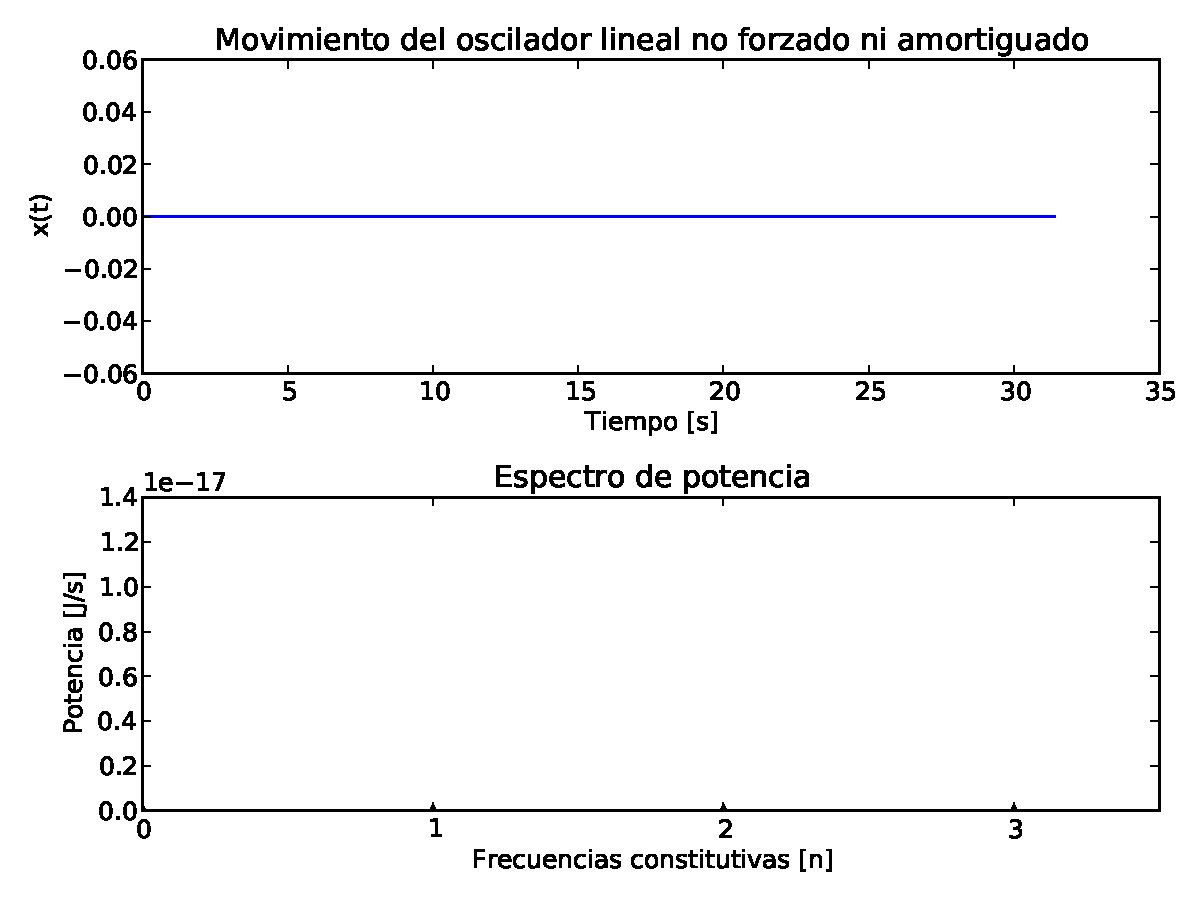
\includegraphics[width=0.75\linewidth]{caso_lineal.pdf}
\caption{Representación de la señal y espectro de potencias para un oscilador lineal no forzado ni amortiguado con $w_o = 1$. La señal ha sido obtenida mediante la aplicación del método de Runge-Kutta de cuarto orden y con un paso de integración $h = 0.01$}
\label{fig:caso_lineal}
\end{figure}

\subsection{Oscilador lineal forzado pero no amortiguado}
Eliminando los términos cuyos coeficientes son cero, el sistema de ecuaciones queda de la siguiente manera

\begin{equation}
	\frac{dx}{dt} = y = f(t, x, y)
\end{equation}

\begin{equation}
	\frac{dy}{dt} = F_o\cos{wt} - w_o^2 x = g(t, x, y) 	
\end{equation}

al que se aplican las condiciones iniciales. El oscilador se encuentra en reposo y en el origen de coordendas, sin embargo, la aplicación de la fuerza oscilante externa con una frecuencia igual a la frecuencia natural del oscilador produce el fenómeno conocido como \textit{resonancia}. Dicha fuerza externa proporciona energía al oscilador produciendo aumentando la amplitud de su movimiento en cada ciclo, efecto puede observarse en la figura \ref{fig:caso_forzado}. En el espectro de potencias pueden observarse varias frecuencias constitutivas que proporcionan la forma de la señal. Una señal sinusoidal pura y de extensión infinita estaría constituida por una única componente de una frecuencia determinada, sin embargo dicha señal no puede representarse en un número finito de ciclos. La señal analizada tiene una longitud determinada en el tiempo y por lo tanto es necesario que esté constituida por varias frecuencias que posibiliten sintetizar la forma adecuada.

\begin{figure}
\centering
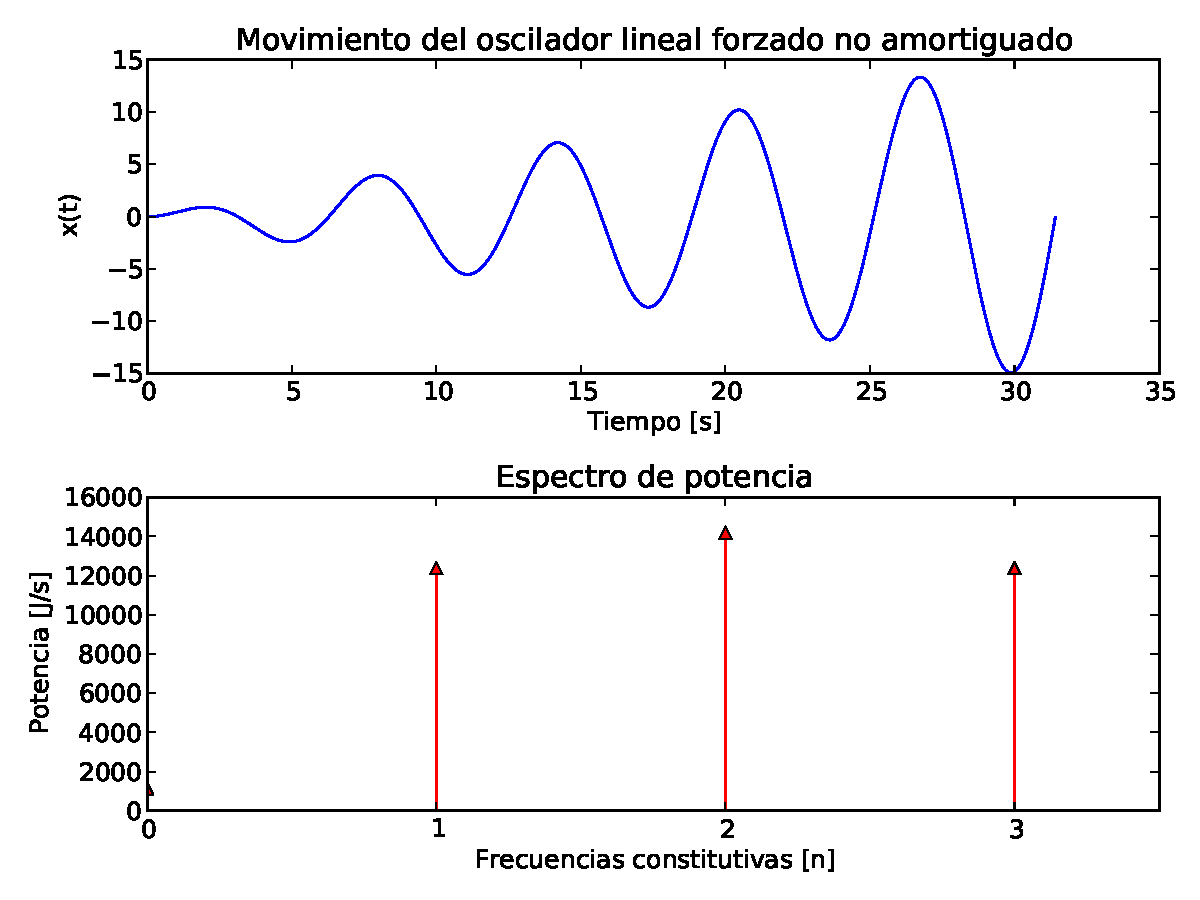
\includegraphics[width=0.75\linewidth]{caso_forzado.pdf}
\caption{Representación de la señal y espectro de potencias para un oscilador lineal forzado pero no amortiguado con $w_o = 1$ y $w = 1$ y un coeficiente para la fuerza $F_o = 1$. La señal ha sido obtenida mediante la aplicación del método de Runge-Kutta de cuarto orden y con un paso de integración $h = 0.01$.}
\label{fig:caso_forzado}
\end{figure}

\subsection{Oscilador lineal forzado y amortiguado}
En el caso de este tipo de oscilación se introduce un nuevo termino en el sistema de ecuaciones que produce una disminución de la energía del oscilador con el paso del tiempo.

\begin{equation}
	\frac{dx}{dt} = y = f(t, x, y)
\end{equation}

\begin{equation}
	\frac{dy}{dt} = F_o\cos{wt} - w_o^2 x - \gamma{}y = g(t, x, y) 	
\end{equation}

A partir de la aplicación de las condiciones iniciales y del método de integración se obtiene la señal correspondiente al oscilador armónico forzado y amortiguado. Como puede observarse en la figura \ref{fig:caso_forzado_amortiguado}, la amplitud del movimiento del oscilador no crece de una forma indefinida debido a la aplicación de la fuerza periódica externa, como si ocurre en el caso del oscilador forzado y no amortiguado.

La introducción del factor de amortiguamiento, debido a la aplicación de fuerzas no conservativas, produce la reducción de la energía disponible. Sin embargo, debido a que tanto la fuerza periódica aplicada como la amortiguación son constantes en el tiempo, y una vez que se termina la fase transitoria del inicio del movimiento, el oscilador produce una señal sinusoidal de amplitud constante. Esto puede observarse al analizar el espectro de frencuencias, y comprobar que la forma del espectro de frecuencias es similar al caso anterior. Sin embargo, la potencia de cada componente de frecuencia es menor que el caso en el que no se produce amortiguación, debido a que la amplitud de la señal se encuentra acotada y, por lo tanto, no crece de forma indefinida.

\begin{figure}
\centering
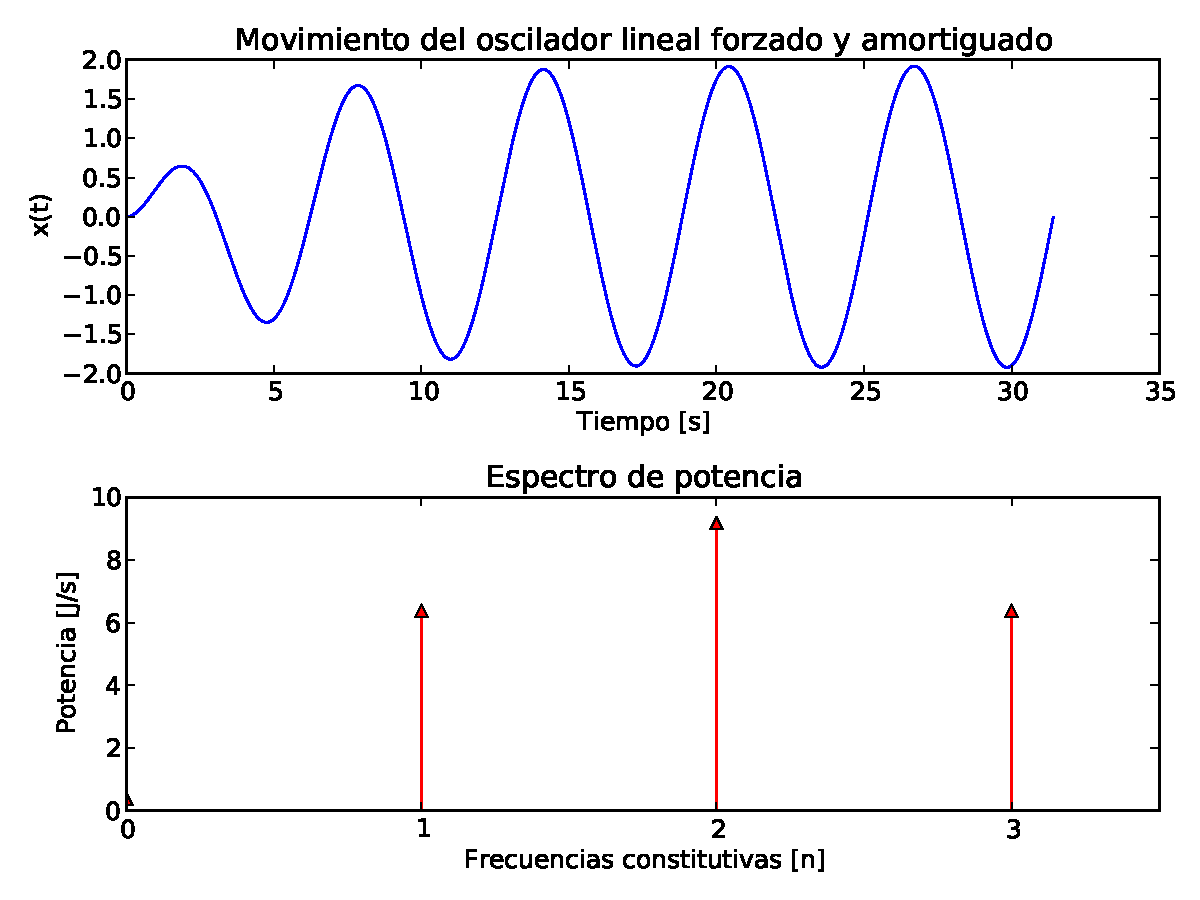
\includegraphics[width=0.75\linewidth]{caso_forzado_amortiguado.pdf}
\caption{Representación de la señal y espectro de potencias para un oscilador lineal forzado y amortiguado con $w_o = 1$, $w = 1$, $F_o = 1$ y un coeficiente de amortiguamiento de $\gamma = 0.52$. La señal ha sido obtenida mediante la aplicación del método de Runge-Kutta de cuarto orden y con un paso de integración $h = 0.01$}
\label{fig:caso_forzado_amortiguado}
\end{figure}

\subsection{Oscilador no lineal forzado y amortiguado}
En este último caso se utiliza la forma completa del sistema de ecuaciones diferenciales que rige el movimiento del oscilador anarmónico:

\begin{equation}
	\frac{dx}{dt} = y = f(t, x, y)
\end{equation}

\begin{equation}
	\frac{dy}{dt} = F_{o}\cos{\omega{}t} -\gamma{}y - \omega_{o}^2x - \beta{}x^2 = g(t, x, y) 	
\end{equation}

utilizando nuevamente las condiciones iniciales y aplicando los métodos numéricos correspondientes se obtiene la señal correspondiente a este oscilador. Se estudian dos conjuntos diferentes de parámetros:

\begin{itemize}
	\item S1: $\gamma = 0.52$, $F_o = 0.516$, $w = 1.2$
	\item S2: $\gamma = 0.48$, $F_o = 0.5162$, $w = 1.3$
\end{itemize}

Además, en ambos casos se ha utilizado un valor para parámetro $\beta=1.09$ con objeto de obtener un comportamiento aperiódico claro en una representación en pocos periodos.

\subsubsection{Conjunto de parámetros S1}
Al utilizar la configuración de parámetros dada y aplicar el método de resolución de ecuaciones diferenciales de Runge-Kutta al sistema de ecuaciones diferenciales se ha constatado que existe un problema en el mismo: la ecuación es inestable y al llegar a cierto instante de tiempo se produce un estallido y un crecimiento muy rápido que produce valores númericos no representables. En la figura \ref{fig:caso_anarmonico_s1} se observa la representación obtenida hasta que se produce el comportamiento inestable detectado. En esta situación es imposible calcular un número suficiente de periodos que permita aplicar el análisis del espectro de potencias llevado a cabo en los casos anteriores.

La detección del comportamiento anómalo de la función se ha implementado comprobando si en algún momento se obtiene un valor para $x(t)$ definido como NaN. Esto significa que la ecuación se ha vuelto inestable y ha comenzado a crecer en magnitud de forma descontrolada. Esto puede comprobarse en los listados de código incluidos en el anexo al trabajo.

Con objeto de resolver el problema se ha probado a modificar el tamaño del paso de integración, pero no se han obtenido resultados satisfactorios. La inestabilidad en el sistema de ecuaciones se debe a la introducción del factor no lineal en la ecuación y a su correspondiente coeficiente, que produce que dicho término crezca de una forma mucho más rápida que los otros. Las ecuaciones que contienen términos de este tipo se conocen como \textit{ecuaciones rígidas}. 

La solución al problema de la rigidez de las soluciones pasa por la utilización de otros métodos numéricos que tengan produzcan un comportamiento más estable en las ecuaciones integradas. Por ejemplo, se ha comprobado en internet que existen métodos como el 
\textit{Backward Euler Method} y que podría ser posible aplicarlo a sistemas de ecuaciones diferenciales. El método es similar al método de Euler, pero utiliza un representación impĺícita de la función diferencial que debe ser resuelta como un sistema de ecuaciones, en el caso lineal. Sin embargo, el autor de este trabajo no ha conseguido representar correctamente el sistema de ecuaciones diferenciales en la forma necesaria para la aplicación del método. 

\subsubsection{Conjunto de parámetros S2}
Al utilizar el segundo conjunto de parámetros ha sido posible calcular un número de periodos suficiente como para llevar a cabo la integración de la señal durante los periodos necesarios para realizar el análisis de frecuencia promediado. Además, se ha llevado a cabo análisis de Fourier utilizando una frecuencia de señal de $w=1.3$, igual a la de la fuerza periódica externa aplicada al oscilador.

En este caso puede observarse que aparece una nueva componente de frecuencia 0 que es debida al comportamiento no periódico de la función de onda analizada.

\begin{figure}
\centering
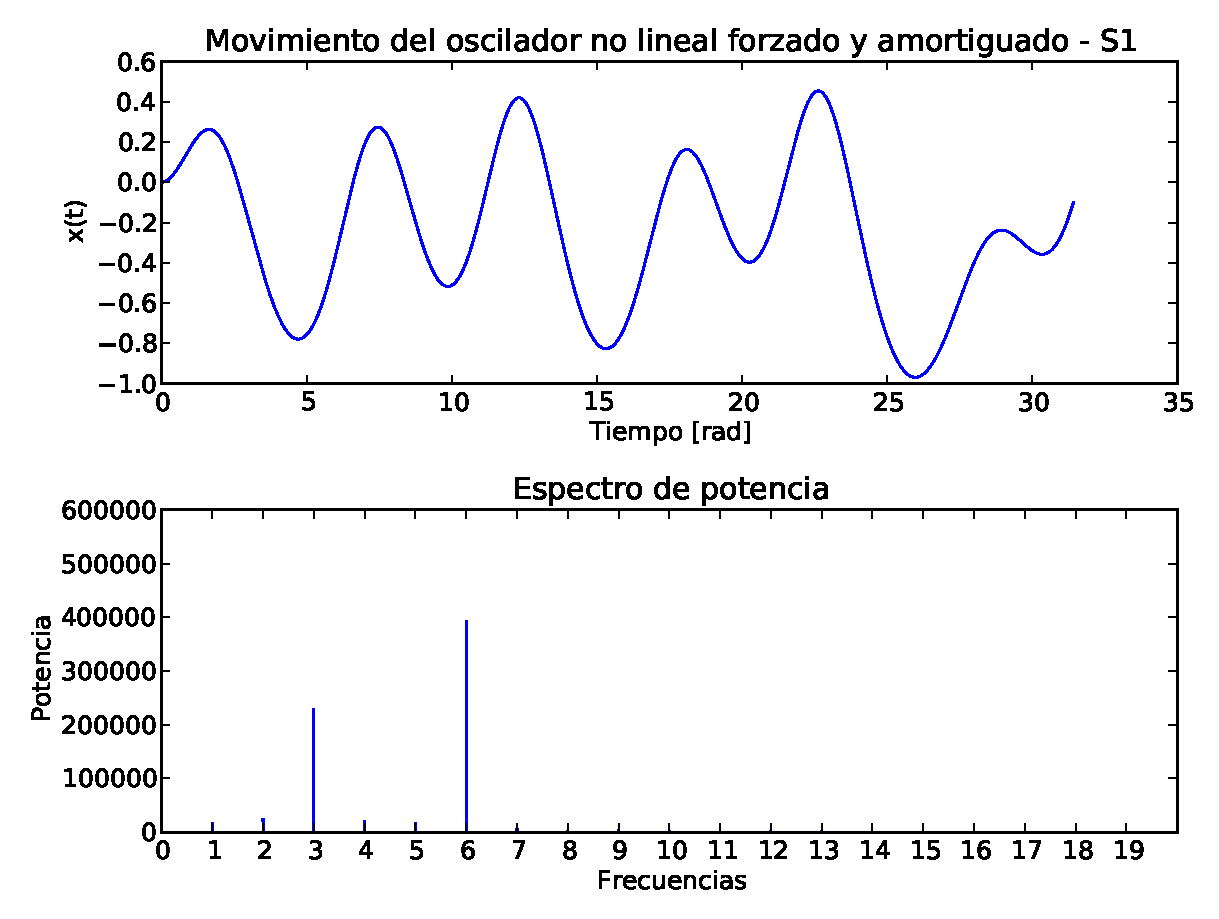
\includegraphics[width=0.75\linewidth]{caso_anarmonico_s1.pdf}
\caption{Representación de la señal y espectro de potencias para un oscilador anarmónico forzado y amortiguado con $w_o = 1$, $w = 1$, $\gamma = 0.52$, $F_o = 0.516$, $w = 1.2$. La señal ha sido obtenida mediante la aplicación del método de Runge-Kutta de cuarto orden y con un paso de integración $h = 0.01$}
\label{fig:caso_anarmonico_s1}
\end{figure}

\begin{figure}
\centering
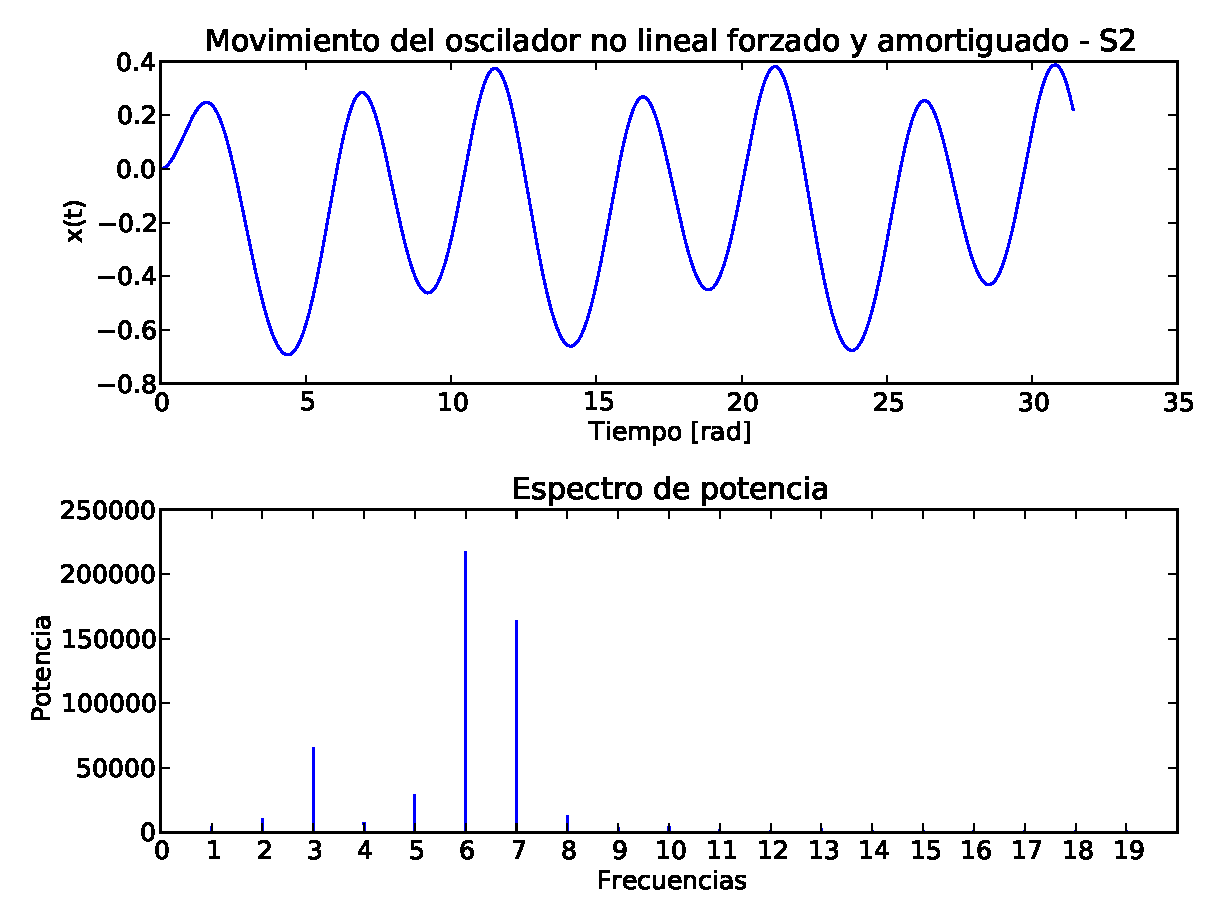
\includegraphics[width=0.75\linewidth]{caso_anarmonico_s2.pdf}
\caption{Representación de la señal y espectro de potencias para un oscilador anarmónico forzado y amortiguado con $w_o = 1$, $w = 1$, $\gamma = 0.48$, $F_o = 0.5162$, $w = 1.3$. La señal ha sido obtenida mediante la aplicación del método de Runge-Kutta de cuarto orden y con un paso de integración $h = 0.01$}
\label{fig:caso_anarmonico_s2}
\end{figure}

\section{Conclusiones}
La realización de este trabajo ha servido para comprobar el funcionamiento real de un método de integración aplicado a un sistema de ecuaciones diferenciales. Ha permitido comprobar cómo de importante es la elección del paso de integración correcto para obtener una la aproximación requerida del método numérico.

Por otro lado, se ha conocido cuáles son las limitaciones de los métodos de integración de tipo explícito, como el método de Runge-Kutta utilizado, cuando se aplican a ecuaciones rígidas. Aunque no se ha podido comprobar una implementación de un método implícito, se ha comprobado la existencia de este tipo de métodos y su mayor adecuación para la resolución de ecuaciones diferenciales en dichos casos.

Además, el trabajo a permitido estudiar el funcionamiento de la Transformada de Fourier Discreta y, mediante algunas pruebas realizadas durante la realización del trabajo, comprobar que el incremento en el número de muestras de la señal produce un incremento notable en el tiempo de computación de la misma. Aunque no se ha llegado a implementar, se ha comprobado que la solución a este problema es la Tránsformada Rápida de Fourier Discreta mediante la utilización de una implementación de la misma proporcionada por la librería \textit{numpy} para Python.
Se ha comprobado que los resultados obtenidos con la utilización de dicha librería concuerdan con la implementación directa de la transformada discreta, mientras que los tiempos de la primera son muchísimo más pequeños que los del código utilizado en el trabajo.

\pagebreak
\section{Anexos}

\subsection{Implementación de los métodos numéricos}
La implementación de los diferentes métodos numéricos utilizandos en este trabajo ha sido realizada utilizando el lenguaje de programación Python (http://www.python.org/). La generación de las gráficas se ha llevado a cabo utilizando la librería \textit{matplotlib} (http://matplotlib.org/) para este lenguaje de programación. Se incluye a continuación un listado del código de los diferentes métodos numéricos utilizados.

\begin{figure}
\lstinputlisting[language=Python, firstline=22, lastline=66]{../metodos/eq_diferenciales.py}
\caption{Código de la implementación del método Runge-Kutta de cuarto orden para la resolución de un sistema de de dos ecuaciones diferenciales}
\label{runge_kutta_code}
\end{figure}

\begin{figure}
\lstinputlisting[language=Python, firstline=1, lastline=41]{../metodos/transformada_fourier.py}
\caption{Código de la implementación de la Transformada de Fourier Discreta y el muestreo de una señal sobre varios periodos}
\end{figure}

\begin{figure}
\lstinputlisting[language=Python, firstline=43, lastline=83]{../metodos/transformada_fourier.py}
\caption{Código de la Transformada de Fourier Discreta promedio cálculo del espectro de potencia}
\end{figure}

\begin{figure}
\lstinputlisting[language=Python, firstline=1, lastline=28]{../graficas.py}
\caption{Implementación del código para la visualización de la señal y el espectro de potencia.
Se ha utilizado la librería matplotlib para la generación de las gráficas}
\end{figure}

\begin{figure}
\lstinputlisting[language=Python, firstline=29, lastline=61, firstnumber=29]{../graficas.py}
\caption{Continuación de la implementación del código para la visualización de la señal y el espectro de potencia.
Se ha utilizado la librería matplotlib para la generación de las gráficas}
\end{figure}

\begin{figure}
\lstinputlisting[language=Python]{../caso_forzado.py}
\caption{Código del caso lineal no amortiguado ni forzado}
\end{figure}

\begin{figure}
\lstinputlisting[language=Python]{../caso_forzado.py}
\caption{Código del caso lineal forzado pero no amortiguado}
\end{figure}

\begin{figure}
\lstinputlisting[language=Python]{../caso_forzado_amortiguado.py}
\caption{Código del caso lineal forzado y amortiguado}
\end{figure}

\begin{figure}
\lstinputlisting[language=Python]{../caso_anarmonico_forzado_amortiguado_s1.py}
\caption{Código del caso no lineal forzado y amortiguado para parámetros S1}
\end{figure}

\begin{figure}
\lstinputlisting[language=Python]{../caso_anarmonico_forzado_amortiguado_s2.py}
\caption{Código del caso no lineal forzado y amortiguado para parámetros S2}
\end{figure}

\end{document}